\graphicspath{{jorge/}}

\section{Sensitivity Analysis}
\section*{Sensitivity Analysis – Questions}

The objective of this analysis is to determine to what extent the system output, represented by the agent’s estimated performance ($\mu$), varies in response to changes in different inputs or configurations. The aim is to identify which factors have the greatest impact on the agent’s overall performance.

\begin{enumerate}
    \item \textbf{Type of data observation}
    \begin{itemize}
        \item Does the agent achieve better performance using observations in simple115\_v2, pixels, or raw format?
        \item The analysis will determine which type of input allows the model to better understand the environment.
    \end{itemize}

    \item \textbf{Actions used}
    \begin{itemize}
        \item Does using a reduced or extended set of actions significantly affect the agent's performance?
        \item It will be evaluated whether limiting or expanding the action options improves or worsens the agent's ability to make effective decisions.
    \end{itemize}

    \item \textbf{Training techniques}
    \begin{itemize}
        \item How sensitive is the performance ($\mu$) to changes in the training algorithm used?
        \item Comparison among methods such as PPO, A3C, and DQN to identify which achieves higher learning efficiency.
    \end{itemize}

    \item \textbf{Submission frequency and quantity}
    \begin{itemize}
        \item Does the frequency of agent submissions to the evaluation system influence performance?
        \item It will be investigated whether it's more effective to submit agents continuously or only when significant performance improvements are observed.
    \end{itemize}

    \item \textbf{Initial uncertainty ($\sigma$) and early learning}
    \begin{itemize}
        \item How beneficial is it to make multiple submissions during the early training stages compared to later stages?
        \item The goal is to understand whether an early approach helps reduce uncertainty and accelerate rating convergence.
    \end{itemize}

    \item \textbf{Agent policy change (exploration vs exploitation)}
    \begin{itemize}
        \item Do agents with more conservative strategies (exploitation) or more risk-taking strategies (exploration) achieve better results?
        \item This will analyze which approach tends to produce a higher $\mu$ value in the long term.
    \end{itemize}

    \item \textbf{Fatigue, roles, and red cards}
    \begin{itemize}
        \item How useful is it to include this type of additional context in the observations?
        \item It will be assessed whether considering these variables improves the agent’s decisions during gameplay.
    \end{itemize}

    \item \textbf{Goals and goal difference}
    \begin{itemize}
        \item How much does the number of goals or goal difference influence $\mu$ variation?
        \item The aim is to understand whether the final match score directly impacts the rating adjustment.
    \end{itemize}
\end{enumerate}

\section*{Sensitivity Analysis – Hypotheses}

\begin{enumerate}
    \item \textbf{Type of observation}
    \begin{itemize}
        \item Hypothesis: The way environment data is represented significantly affects the model's learning ability.
        \item Expected observation:
        \begin{itemize}
            \item simple115\_v2: allows faster and more efficient learning, with a higher initial $\mu$.
            \item raw: may lead to lower performance if not properly processed.
            \item pixels: requires more episodes and computational resources.
        \end{itemize}
        \item Sensitivity: High – Small changes in data representation can have a considerable impact on performance.
    \end{itemize}

    \item \textbf{Action set used}
    \begin{itemize}
        \item Hypothesis: A broader action set improves the agent’s adaptability in complex situations.
        \item Expected observation:
        \begin{itemize}
            \item Basic actions: quick but limited strategy.
            \item Extended actions: enables more strategic and versatile gameplay.
        \end{itemize}
        \item Sensitivity: Medium – Influences playing style and win probability.
    \end{itemize}

    \item \textbf{Training algorithm}
    \begin{itemize}
        \item Hypothesis: Some algorithms promote better exploration or converge more efficiently.
        \item Expected observation:
        \begin{itemize}
            \item PPO: stable and commonly used as a baseline.
            \item DQN: may struggle in continuous or complex environments.
            \item A3C: can be unstable, but trains policy and value function simultaneously.
        \end{itemize}
        \item Sensitivity: High – Directly affects how the agent learns from the environment.
    \end{itemize}

    \item \textbf{Submission frequency and quantity}
    \begin{itemize}
        \item Hypothesis: The submission strategy influences the agent’s visibility and optimization.
        \item Expected observation:
        \begin{itemize}
            \item Frequent submissions: can quickly rank the best agent.
            \item Selective and optimized submissions: avoid penalties from low-performing agents.
        \end{itemize}
        \item Sensitivity: Medium – Affects the amount and quality of feedback received to improve the model.
    \end{itemize}

    \item \textbf{Initial uncertainty ($\sigma$) and early learning}
    \begin{itemize}
        \item Hypothesis: Early stages are critical for establishing good positioning in the matchmaking system.
        \item Expected observation:
        \begin{itemize}
            \item Early submissions with good performance allow for rapid ranking.
            \item Late submissions may not reach optimal $\mu$ before the competition ends.
        \end{itemize}
        \item Sensitivity: High – Initial uncertainty ($\sigma$) and playtime strongly influence the rating.
    \end{itemize}

    \item \textbf{Play style (exploration vs. exploitation)}
    \begin{itemize}
        \item Hypothesis: Agents with high exploration may discover new strategies but compromise stability.
        \item Expected observation:
        \begin{itemize}
            \item High exploration: generates unexpected behaviors and potential tactical advantages.
            \item Low exploration: produces safer but more predictable behaviors.
        \end{itemize}
        \item Sensitivity: Medium – May be beneficial or detrimental depending on the tournament stage.
    \end{itemize}

    \item \textbf{Fatigue, cards, and player roles}
    \begin{itemize}
        \item Hypothesis: These factors may influence agent behavior, although their impact depends on the model and how the environment penalizes those conditions.
        \item Expected observation: They will only be useful if the agent is advanced enough to learn from these signals.
        \item Sensitivity: Medium – Add value in more complex and context-aware models.
    \end{itemize}

    \item \textbf{Goals and goal difference}
    \begin{itemize}
        \item Observation: The scoring system $\mu$ is based solely on the match result (win, draw, or loss), not on the number of goals.
        \item Sensitivity: Low – Winning by one or many goals does not affect $\mu$ update.
    \end{itemize}
\end{enumerate}

\section*{Visualization of Hypothetical Results (As part of the sensitivity analysis)}

A graph was created based on hypothetical results, constructed from reasonable assumptions consistent with the rating update system rules ($\mu$). This visualization does not use real data but reflects expected behaviors according to the dynamics of the competition environment.

\subsection*{Initial hypothesis:}
The analysis starts with a base value of $\mu$ = 600, common in matchmaking systems like TrueSkill or similar.

It evaluates how different configurations impact the evolution of the estimated rating during the first few days of the competition, within a possible range between 580 and 650.

This range is justified under the assumption that:
\begin{itemize}
    \item Agents are matched against opponents of similar level.
    \item $\mu$ updates after each match are moderate.
    \item In the early days, $\mu$ changes reflect the adaptation and initial learning process.
\end{itemize}

Variables analyzed:
\begin{itemize}
    \item Type of observation (simple115\_v2, raw, pixels)
    \item Training algorithm (PPO, A3C, DQN)
    \item Submission frequency (high vs. low frequency)
\end{itemize}

\begin{figure}
    \centering
    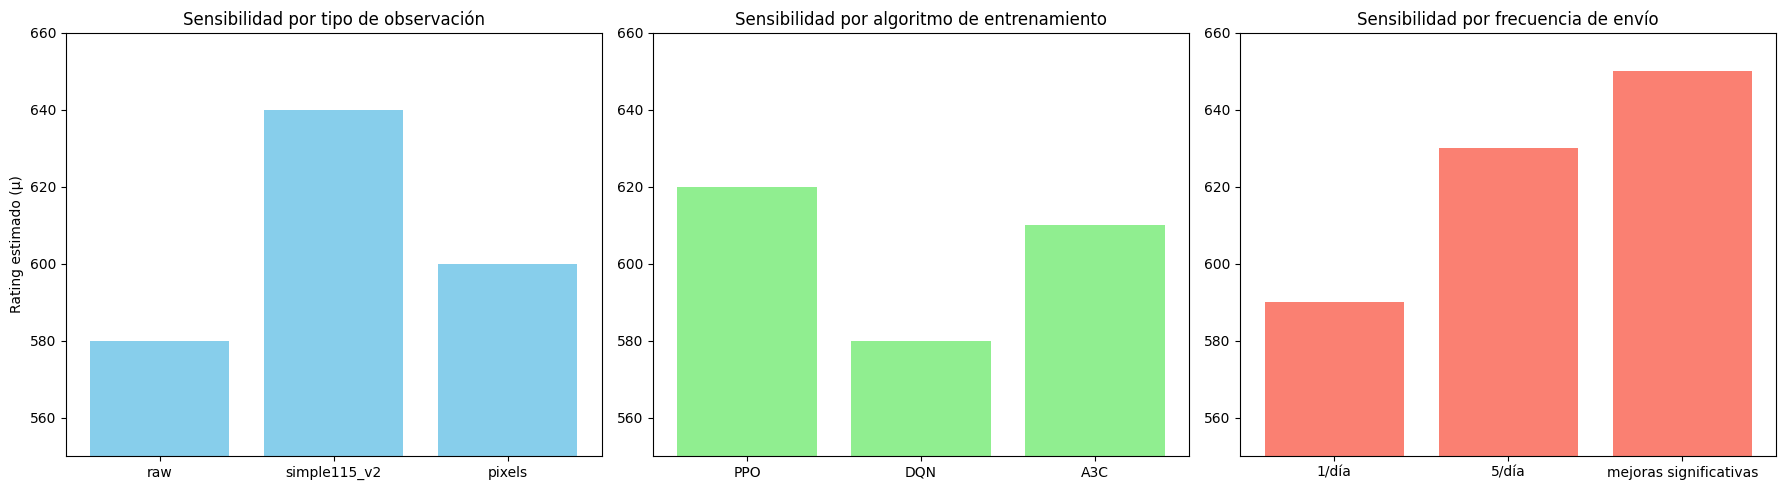
\includegraphics[width=\linewidth]{grafe} 
    \caption{Score Projection Charts}
    \label{fig:enter-label}
\end{figure}


\subsection*{Results Obtained (Graphs):}
The graph shows how, depending on the configuration:
\begin{itemize}
    \item Agents using simple115\_v2 tend to show a faster and more stable growth curve.
    \item Agents trained with PPO display a more consistent progression compared to A3C or DQN.
    \item Frequent submissions allow for quicker adjustments in the system, favoring continuous improvement in $\mu$, while sporadic submissions show less variation in the short term.
\end{itemize}

\section*{Conclusions}

\begin{tabular}{|l|l|l|}
\hline
Variables & Sensitivity & Importance \\
\hline
Training algorithm & High & Affects decisions → Wins → Affects $\mu$ \\
Type of observation & High & More information → Better performance \\
Submission frequency & High & Better $\mu$ estimates and feedback \\
Action set & Medium & Influences the agent’s tactical execution \\
Fatigue, Roles, Cards & Medium & Useful in specific moments \\
Play style & Medium & Specific, infrequent cases \\
Goals/Goal difference & Low & Does not affect $\mu$ updates \\
\hline
\end{tabular}
